\subsection{Long Short-Term Memory}
\label{sub:LSTM}

% Introduction
In 1997, Hochreiter and Schmidhuber introduced a model known as \gls{lstm}. This model addresses the vanishing gradient problem within \glspl{rnn} by incorporating gated activation functions \citep{hochreiter1997long}.
\newline
\newline
% Building blocks
\glspl{lstm} are designed to enhance the memory persistence of \glspl{rnn}, making it easier for them to capture long-term dependencies. All \glspl{rnn} consist of a chain of repeating neural network modules. In standard \glspl{rnn}, these modules are relatively simple, often having only a single \gls{tanh} activation function, as shown in Figure \ref{fig:repeating_modules_rnn}.

\begin{figure}[ht]
    \centering
    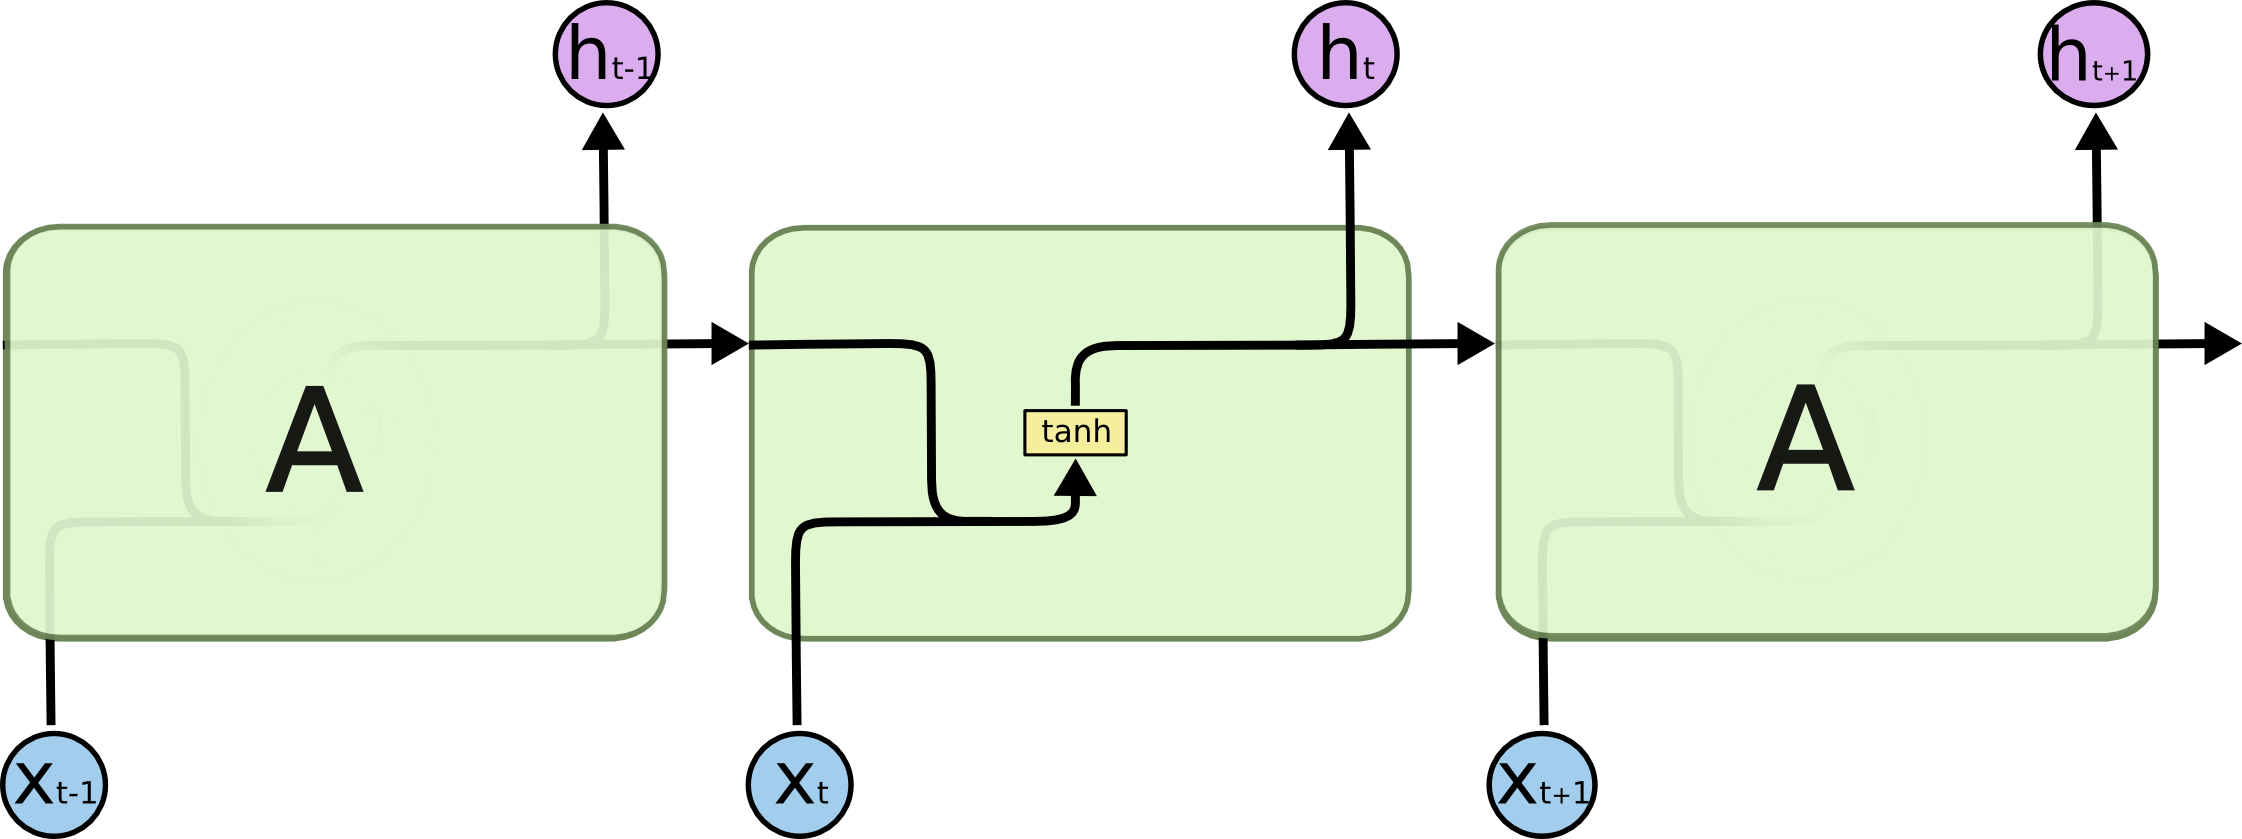
\includegraphics[width=0.75\textwidth]{./assets/img/repeating_modules_rnn.png}
    \caption{The repeating module in a standard \gls{rnn} contains a single layer. Figure from \cite{Olah_2015}.}
    \label{fig:repeating_modules_rnn}
\end{figure}

\noindent
In contrast, \glspl{lstm} also use a chain-like structure, but their repeating module is more complicated. Instead of a single layer, it consists of four interconnected layers, as shown in figure \ref{fig:repeating_modules_lstm}.

\begin{figure}[ht]
    \centering
    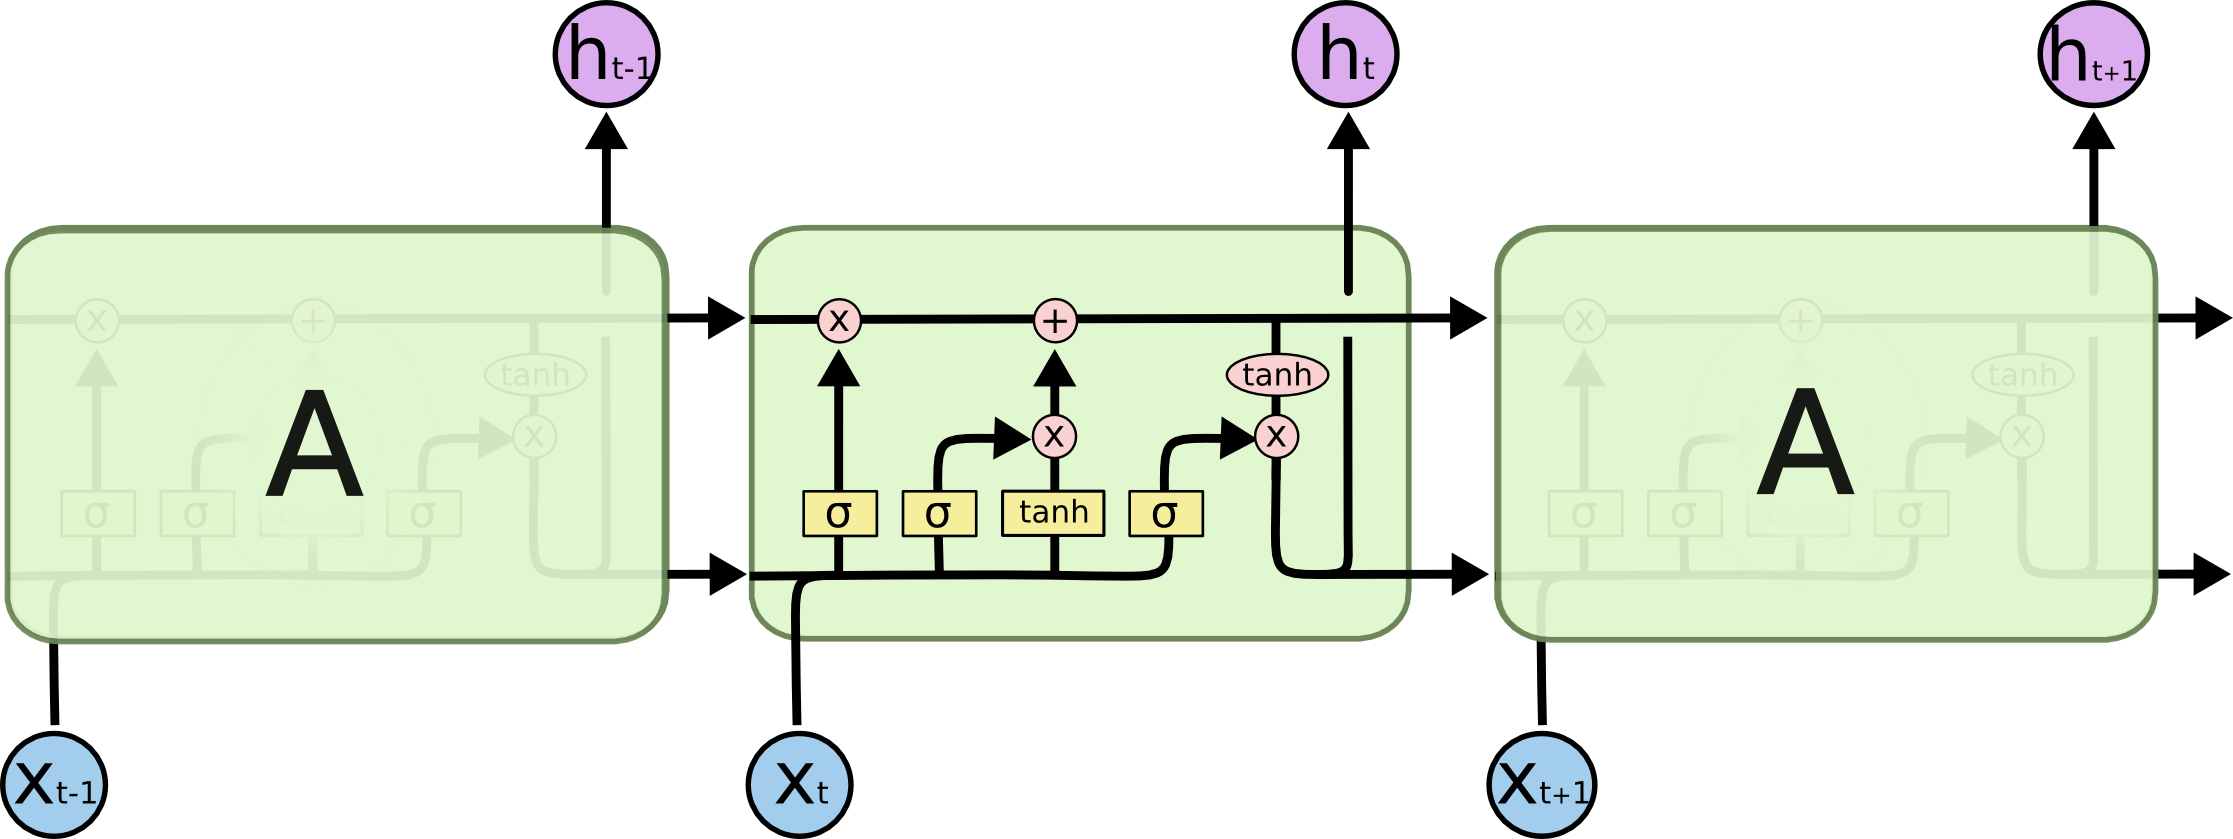
\includegraphics[width=0.75\textwidth]{./assets/img/repeating_modules_lstm.png}
    \caption{The repeating module in a \gls{lstm} contains four interacting layers. Figure from \cite{Olah_2015}.}
    \label{fig:repeating_modules_lstm}
\end{figure}

\noindent
The heart of \glspl{lstm} is the \textit{cell state}, a horizontal line that runs from the left to the right top of the diagram in figure \ref{fig:cell_state_lstm}.

\begin{figure}[ht]
    \centering
    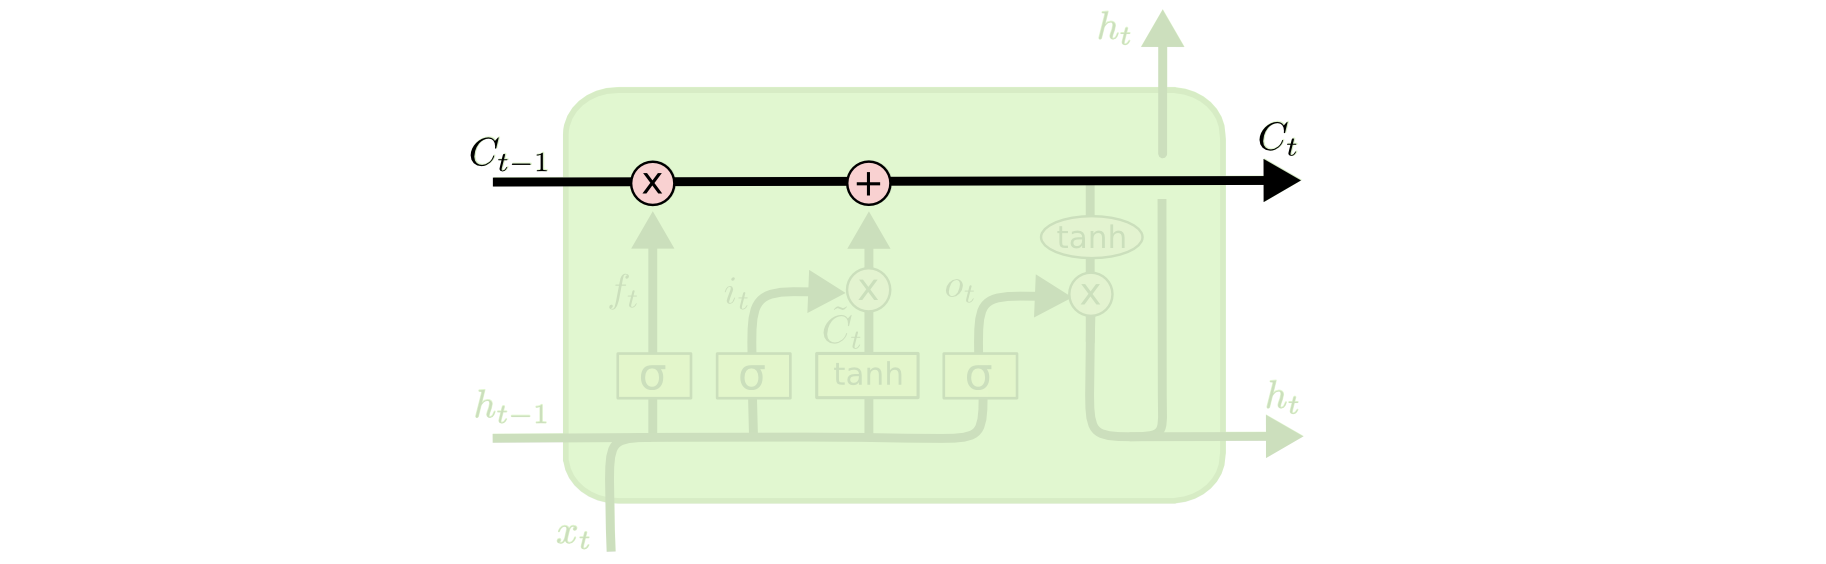
\includegraphics[width=0.85\textwidth]{./assets/img/cell_state_lstm.png}
    \caption{Cell state in \glspl{lstm}. Figure from \cite{Olah_2015}.}
    \label{fig:cell_state_lstm}
\end{figure}

\noindent
The \textit{cell state} runs along the entire chain, allowing information to flow relatively unchanged. The unique feature of the \gls{lstm} network is its ability to selectively remove or add information to the \textit{cell state}, a process controlled by specialised structures called \textit{gates}. \textit{Gates} act as filters, determining which information should pass through. They consist of a sigmoid neural network layer and pointwise multiplication, as illustrated in figure \ref{fig:gates_of_lstms}.

\begin{figure}[ht]
    \centering
    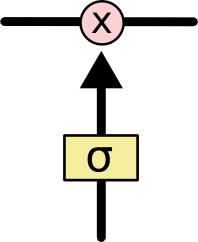
\includegraphics[keepaspectratio,height=3cm]{./assets/img/gates_of_lstms.png}
    \caption{Gates of \glspl{lstm}. Figure from \cite{Olah_2015}.}
    \label{fig:gates_of_lstms}
\end{figure}

\noindent
The sigmoid layer outputs values between zero and one, indicating how much of each component should pass, and can be calculated using the equation from figure \ref{fig:Activation_Functions}. A value of zero implies no information transfer, while a value of one allows everything to pass. \glspl{lstm} integrates three such gates, as shown in figure \ref{fig:lstm_gates}, to control and manage the state of the cell.

\begin{figure}[htb]
    \centering
    \begin{subfigure}{.45\linewidth}
        \centering
        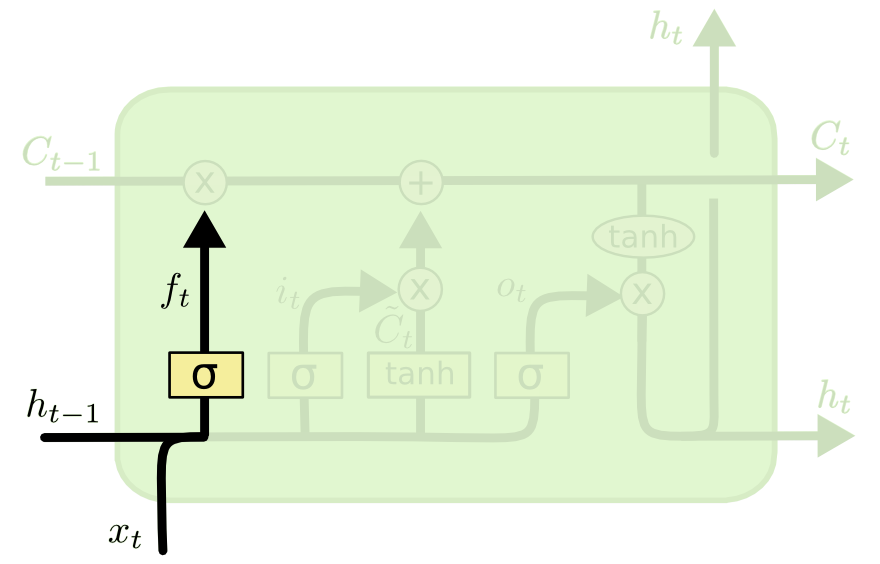
\includegraphics[width=1.0\linewidth]{./assets/img/forget_gate.png}
        \caption{Forget Gate}
        \label{fig:lstm_forget_gate}
    \end{subfigure}
        \begin{subfigure}{.45\linewidth}
        \centering
        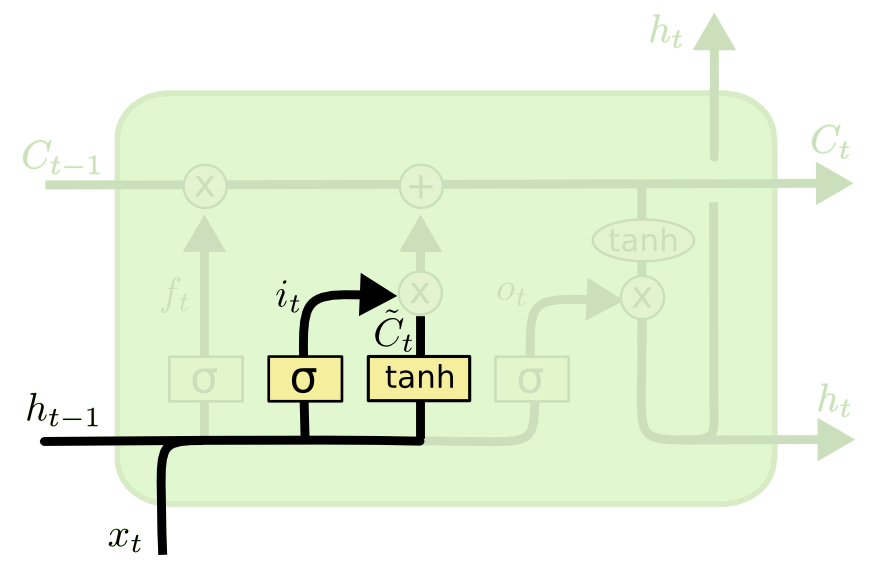
\includegraphics[width=1.0\linewidth]{./assets/img/input_gate.png}
        \caption{Input Gate}
        \label{fig:lstm_input_gate}
    \end{subfigure}
        \begin{subfigure}{.45\linewidth}
        \centering
        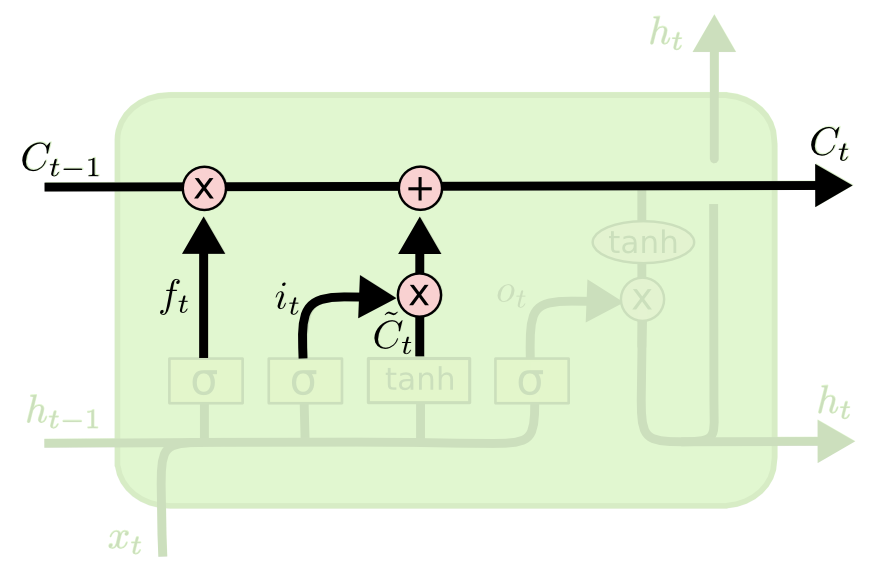
\includegraphics[width=1.0\linewidth]{./assets/img/update_gate.png}
        \caption{Update Gate}
        \label{fig:lstm_update_gate}
    \end{subfigure}
        \begin{subfigure}{.45\linewidth}
        \centering
        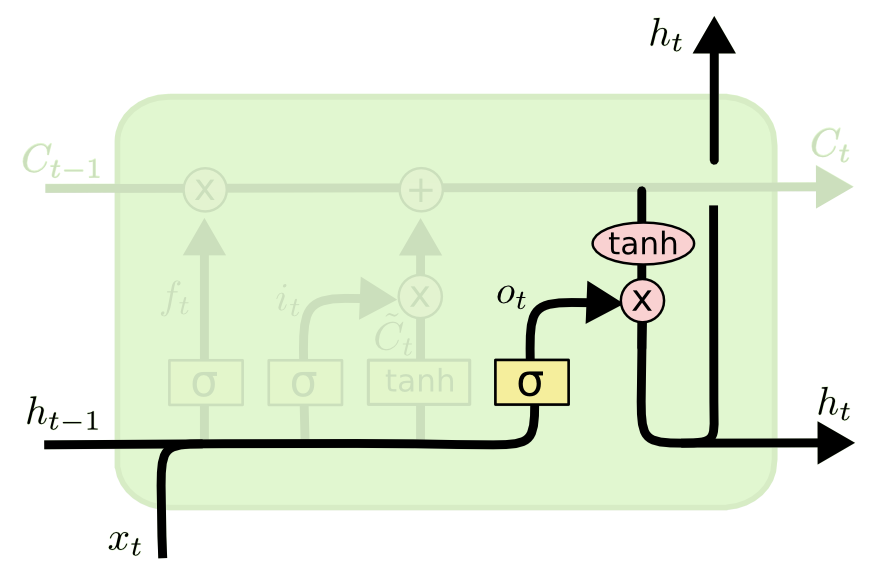
\includegraphics[width=1.0\linewidth]{./assets/img/output_gate.png}
        \caption{Output Gate}
        \label{fig:lstm_output_gate}
    \end{subfigure}
    \caption{The four \gls{lstm} gates. Figure from \cite{Olah_2015}}
    \label{fig:lstm_gates}
\end{figure}

\noindent
% Gates step-by-step
The first gate, known as the \textit{forget gate} (figure \ref{fig:lstm_forget_gate}), determines which information in the cell state should be discarded. It calculates the output using the equation \ref{eq:calculation_forget_gate}.

\myequations{Calculating the output of the forget gate}
\begin{equation}
    \centering
    f_t = \sigma \left(W_f \cdot [h_{t-1}, x_t] + b_f \right)
    \label{eq:calculation_forget_gate}
\end{equation}

\noindent
The second gate, the \textit{input gate} (figure \ref{fig:lstm_input_gate}), controls the addition of new information to the \textit{cell state}. This gate has two parts: the first, a sigmoid layer called the \textit{input gate layer}, determines which values to update, as shown in equation \ref{eq:input_gate}. Next, a \gls{tanh} layer generates a vector of new candidate values ($\tilde{C}_t$) that could be incorporated into the state, according to the equation \ref{eq:candidates_cell_state}.

\myequations{Calculating the decision of new inputs}
\begin{equation}
    \centering
    i_t = \sigma \left(W_i \cdot [h_{t-1}, x_t] + b_i \right)
    \label{eq:input_gate}
\end{equation}

\myequations{Calculating the candidates for the cell state}
\begin{equation}
    \centering
    \tilde{C}_t = \text{tanh} \left(W_C \cdot [h_{t-1}, x_t] + b_C \right)
    \label{eq:candidates_cell_state}
\end{equation}

\noindent
Subsequently, the \textit{update gate} (figure \ref{fig:lstm_update_gate}) modifies the old \textit{cell state} ($\tilde{C}_{t-1}$) to obtain the new \textit{cell state} ($\tilde{C}_t$) according to equation \ref{eq:update_cell_state}. It combines the effect of the forget gate (as calculated in equation \ref{eq:calculation_forget_gate}) and the decision of the input gate.

\myequations{Updating the cell state}
\begin{equation}
    \centering
    \tilde{C}_t = f_t \cdot \tilde{C}_{t-1} + i_t \cdot \tilde{C}_{t}
    \label{eq:update_cell_state}
\end{equation}

\noindent
Finally, the \textit{output gate} (figure \ref{fig:lstm_output_gate}) also has two components: the first, governed by the equation \ref{eq:output_gate_sigmoid}, calculates the information from the input that should be used, applying a sigmoid activation function. This result is then multiplied by the information from the cell state passing through a \gls{tanh} layer, as shown in equation \ref{eq:output_gate_tanh}.

\myequations{Sigmoid activation output gate}
\begin{equation}
    \centering
    o_t = \sigma \left( W_o [h_{t-1,x_t}] + b_o \right)
    \label{eq:output_gate_sigmoid}
\end{equation}

\myequations{Updating the cell state}
\begin{equation}
    \centering
    h_t = o_t \cdot \text{tanh}(C_t)
    \label{eq:output_gate_tanh}
\end{equation}